\documentclass{bioinfo}
\copyrightyear{2005}
\pubyear{2005}
\usepackage{graphicx}
\hyphenation{Complex-Assembly}
\begin{document}
\firstpage{1}

\title[BioPax to SBML qual]{Qualitative translation of relations from BioPax to SBML qual}
\author[B\"uchel \textit{et~al}]{Finja B\"uchel\,$^{1,*}$,
and Andreas Zell\,$^1$\footnote{to whom correspondence should be addressed}}
\address{$^{1}$Department of Cognitive Systems, University of Tuebingen, Sand 1, 72076 T\"ubingen, Germany\\}


\history{Received on XXXXX; revised on XXXXX; accepted on XXXXX}

\editor{Associate Editor: XXXXXXX}

\maketitle

\begin{abstract}

\section{Motivation:}
BioPax and SBML are the two most popular modeling and data exchange languages in systems biology. The focus of SBML is quantitative modeling and dynamic simulation of molecular interaction pathways, whereas the BioPax specification concentrates on visualization and qualitative analysis of pathway maps. BioPax models reactions and relations. In contrast, SBML is exclusively able to handle reactions. But with the release of the SBML qualitative Models extension (qual), it has recently also become possible to describe relations in SBML. Before this release, relations could not be translated to SBML or were erroneously converted to reactions. Until now, there exists no converter for BioPax to SBML, that is fully capable to translate both reactions and relations.
\section{Results:}
Here we present the conversion of the complete nature Pathway Interaction Database (PID) which includes pathways from BioCarta, Reactome, and from the National Cancer institute. PID provides the pathways in the BioPax Level 2 and Level 3 format. Both formats are translated to the SBML format including the new qual extension. Thus, the result SBML files contain both reactions and relations.
\section{Availability:}
The complete collection of the PID models is freely available on our homepage ..... (\textbf{TODO Finja: create homepage! and and if necessary licence})
\section{Contact:} \href{finja.buechel@uni-tuebingen.de}{finja.buechel@uni-tuebingen.de}
\end{abstract}

\section{Introduction}
The goal of systems biology is the modeling and understanding of biological and chemical processes in a cell. BioPax and SBML are common modeling languages to describe such processes. The BioPax specification aims at exchanging, visualization, and analyzing such processes on a large scale. BioPax can be used to image metabolic, signaling, molecular, gene regulatory and genetic interaction networks \citep{Demir2010}. In contrast, SBML is mostly used for quantitative modeling because it offers the possibility to include kinetic equations and enables the interpretation of the interaction network as an differential equation system \citep{Hucka2003}. This is due to a detailed and comprehensive SBML specification which additionally facilitates software support for investigation and simulation processes \citep{Draeger2008}. The SBML core specification defines reactions in detail but no other relationships between molecules.
%problem
Before the release of the qualitative model specification (qual), it was not possible to define relations or to integrate reactions and relations in one model (\textbf{cite qual?}).
%relevance
Furthermore, it was not possible to easily combine or exchange information between different databases, if one database uses the BioPax format and the other one the SBML format.
%literature review
So far, there exist several visualization tools, like Cytoscape or CellDesigner, which can handle both formats by using plugins \citep{Mi2011, Draeger2008, Funahashi2007, Smoot2011a, Zinovyev2008}). \citet*{Ruebenacker2009} suggest a new a bridging format to solve the problem of the conversion from BioPax to SBML. But until now, there exists only converters from SBML to BioPax like The System Biology Format Converter (see http://www.ebi.ac.uk/compneur-srv/sbml/converters/SBMLtoBioPax.html) but no converter for BioPax to SBML, whose conversion would also include relations. The need to combine both formats to use the knowledge different databases in various application becomes more and more urgent.\\
% what we did
% necessary to mention why we use PID?
In this paper we present a complete conversion of the nature Pathway Interaction Database (PID, \citet{Schaefer2009}) from BioPax Level 2 and Level 3 format to the SBML format including the qual extension. The pathway conversion is implemented in Java (\textbf{TODO: Java Trademark}) and uses JSBML \citep{Draeger2011} and PaxTools \citep{Demir2010}. The translated files are freely available on our homepage: ...\textbf{TODO and add licence}
% what we find out
% what do the results mean (why are they significant?)

\textbf{TODO: Clemens, Florian und Andreas: Habt ihr hier noch konkrete Ideen, was ich noch einbauen k\"onnte? Fehlt etwas?}


\begin{methods}
\section{Material and Methods}
\subsection{The SBML and the qualitative Models extension}
%%%%%%%%% SBML
The SBML (Systems Biology Markup Language) core specification is a special XML format to describe quantitative models. Therefore, several classes are defined describing molecules and their interaction in a model. The most important class \textbf{(TODO: better word, because SBase is an interface)} is \texttt{SBase} which inherits \texttt{species}, \texttt{reaction} and several other elements. A \texttt{species} element describe each kind of molecule and can be further determined with the aid of annotations, like MIRIAM (\textbf{TODO: cite? more description?, Are there other annotations like GO?}). The SBML core specification provides no possiblitiy itself to define other relationships than concrete quantitative reactions. \citep{Hucka2003}\\
%%%%%%%%% SBML qual
The SBML qualitative models extension (qual) introduces qualitative elements, such as \texttt{qualitativeSpecies}, \texttt{symbol}, and \texttt{transition}, providing the necessary means to describe relationships like enzyme-enzyme relations, protein-protein interactions, interactions of transcription factors and genes, protein-compound interaction, or links to other pathways.
%Although, technically, those processes are chemical reactions, too, it can often be far more useful to represent them by logical states and transitions. (\textbf{TODO: Florian k�nntest du den Satz etwas positiver formulieren, mir ist die Intention nicht ganz klar})
Instead of concentration levels that are transformed continuously via reactions, \texttt{qualitativeSpecies} have discrete states that are changed using \texttt{transition}s.
These \texttt{transitions} consist of \texttt{input} and \texttt{output} elements and at least one \texttt{functionTerm}.
If, in a qualitative model, a protein A is inhibiting a protein B, this would be represented as a \texttt{transition} with \texttt{input} A and \texttt{output} B.
Furthermore, the input element has a \texttt{sign} attribute which describes if the relationship between the input and output elemenst is \texttt{positive}, \texttt{negative}, \texttt{dual}, or \texttt{unknown}.
%models beschreiben

\subsection{The BioPax specification}
BioPax, the Biology Pathway Exchange Language, is an OWL (Web Ontology Language) dialect which based on the RDF syntax. There is one super class called \texttt{entity} which extends all other BioPax classes. One distinguishes between two main classes: \texttt{PhysicalEntity} and \texttt{interaction}. \texttt{PhysicalEntity} describes molecules, like proteins, complexes, small molecules, DNA, or RNA, whereas \texttt{Interaction} defines reactions and relations between the \texttt{PhysicalEntity}s. \texttt{Interaction} is split into \texttt{Control} and \texttt{Conversion} which can be separated into the subclasses \texttt{Catalysis}, \texttt{Modulation}, \texttt{Transport}, \texttt{BiochemicalReaction}, and \texttt{Complex\-Assembly}.\\
BioPax is released level-wise. The current level is level 3. Level 1 is exclusively able to describe metabolic interactions, whereas in Level 2 additionally supports signaling pathways and molecular interactions. The difference between level 2 to level 3 is the ability of level 3 to model gene regulatory networks and genetic interactions. For this purpose the control subclass \texttt{TemplateReactionReglulation} and the conversion subclass \texttt{Degradation} are added. Furthermore, \texttt{PhysicalEntity} is now able to define \texttt{DNAregion} and \texttt{RNAregion}.
Level 3 is not backwards compatible with Level 2, but Level 2 is backward compatibel with Level 1. \citep{Demir2010}
\subsection{Conversion of BioPax to SBML qual}
%%%%%%%%% Material and implementation
The complete the nature Pathway Interaction Database (PID) is converted from BioPax Level 2 and Level 3 to SBML including the qualitative models extension (\citep{Schaefer2009}). PID provides NCI-Nature curated pathways, pathways from BioCarta from June 2004, and Reactome human pathways from Verstion 22, whereas the Reactome data is updated as soon as new pathway informations are available. \\
The conversion was programmed with Java, using JSBML \citep{Draeger2011} with the qualitative models extension, PaxTools. and the KEGG API (\textbf{TODO: citation?}). PaxTools was used to read the BioPax files and to manipulate the information content. This information was extended (\textbf{TODO Clemens: Welche Info haven wir aus der KEGG-API?}) using the KEGG API, and finally the transformed information was written with the use of JSBML classes.\\

% determining the organism
% determining the pathway content
% conversion of Entities, gene id...
% conversion of reaction
% conversion of relations

\begin{itemize}
\item Species(Organism) is determined automatically (if it is mentioned in the file)
\item Works file vice, 1 file = 1 pathway
\item how is distinguished between a transition and a reaction... -> include table
\item gene symbol -> gene id -> unknown
\item annotations of the species? \textbf{TODO Clemens: K\"onntest du das bitte ausf\"uhren/erg\"anzen?SBO terms, GO,...?}
\end{itemize}


\begin{table}[!t]
\processtable{Description of the translation of BioPax control elements\label{Tab:BioPax2SBML}}
{\begin{tabular}{llll}\toprule
BioPax controller & BioPax controlled               & Converted\\
                  &                                 & SBML qual\\
                  &                                 & element\\
\midrule
\textbf{BioPax Level 3}\\
\midrule
PhysicalEntity & BiochemicalReaction                & reaction\\
PhysicalEntity & ComplexAssembly                    & reaction\\
PhysicalEntity & Control                            & transition\\
PhysicalEntity & Degradation                        & transition\\
PhysicalEntity & Transport                          & transition\\
PhysicalEntity & TransportWithBiochemicalReaction   & reaction\\
PhysicalEntity & Pathway                            & transition\\
PhysicalEntity & TemplateReaction                   & transition\\
\\
Pathway         & BiochemicalReaction               & transition\\
Pathway         & ComplexAssembly                   & transition\\
Pathway         & Control                           & transition\\
Pathway         & Degradation                       & transition\\
Pathway         & Pathway                           & transition\\
Pathway         & TemplateReaction                  & transition\\
Pathway         & Transport                         & transition\\
Pathway         & TransportWithBiochemicalReaction  & transition\\
\\\midrule
\textbf{BioPax Level 2}\\
\midrule
physicalEntity & biochemicalReaction                & reaction\\
physicalEntity & complexAssembly                    & reaction\\
physicalEntity & control                            & transition\\
physicalEntity & pathway                            & transition\\
physicalEntity & transport                          & transition\\
physicalEntity & transportWithBiochemicalReaction   & reaction\\
\\
pathway         & biochemicalReaction               & transition\\
pathway         & complexAssembly                   & transition\\
pathway         & control                           & transition\\
pathway         & pathway                           & transition\\
pathway         & transportWithBiochemicalReaction  & transition\\
pathway         & transport                         & transition\\\botrule
\end{tabular}}{BioPax control elements consists of a controller and one or more controlled elements. Depending on the kind of controller or controlled element, an entity is translated to a reaction or a transition. The table gives an overview of this conversion regarding BioPax Level 2 and BioPax Level 3.}
\end{table}



%%%%%%%%%%%%%%%%%%%%%%%%%%%%%
%% CLEMENS: MIRIAM und SBO %%
%%%%%%%%%%%%%%%%%%%%%%%%%%%%%
The BioPax specification allows users to encode arbitrary identifiers for elements. These can be identifiers for various databases, e.g., UniProt, Entrez Gene, Ensembl, etc. Unfortunately, the syntax used in BioPax is not very consistent which leads to XML elements like TODO-X or TODO-Y within BioPax documents that hamper the automatic reading and interpretation of those models by third party applications. [FINJA: BITTE DIE TODOS MIT DEM BEISPIEL <RDF UNIPROT=UNIPROT:hj35k3> und <RDF UNIPROT=hj35k3> oder \"ahnlichen uneinheitlichen beispielen f\"ullen]
In SBML, such identifiers can be expressed as standardized MIRIAM URNs that can be added as annotation to any SBML element. We support and add MIRIAM identifiers for the following databases: Entrez Gene, Omim, Ensembl, UniProt, ChEBI, DrugBank, Gene Ontology, HGNC, PubChem, 3DMET, NCBI Taxonomy, PDBeChem, GlycomeDB, LipidBank, EC-Numbers (enzyme nomeclature) and various KEGG databases (gene, glycan, reaction, compound, drug, pathway, orthology).
All supported identifiers from the BioPax files are parsed, some are manually curated (see example of inconsistent usage above) and many annotations are supplemented by additional queries to the KEGG API for every translated element. The goal of those annotations is to provide models that can be used directly by many researchers, no matter what identifiers or databases they use.

TODO: Typen (protein, gen, etc.) als SBO term in detail auflisten und erklaeren.
%%%%%%%%%%%%%%%%%%%%%%%%%%%%%
%%%%%%%%%%%%%%%%%%%%%%%%%%%%%
\begin{figure*}[t!h]
\centering 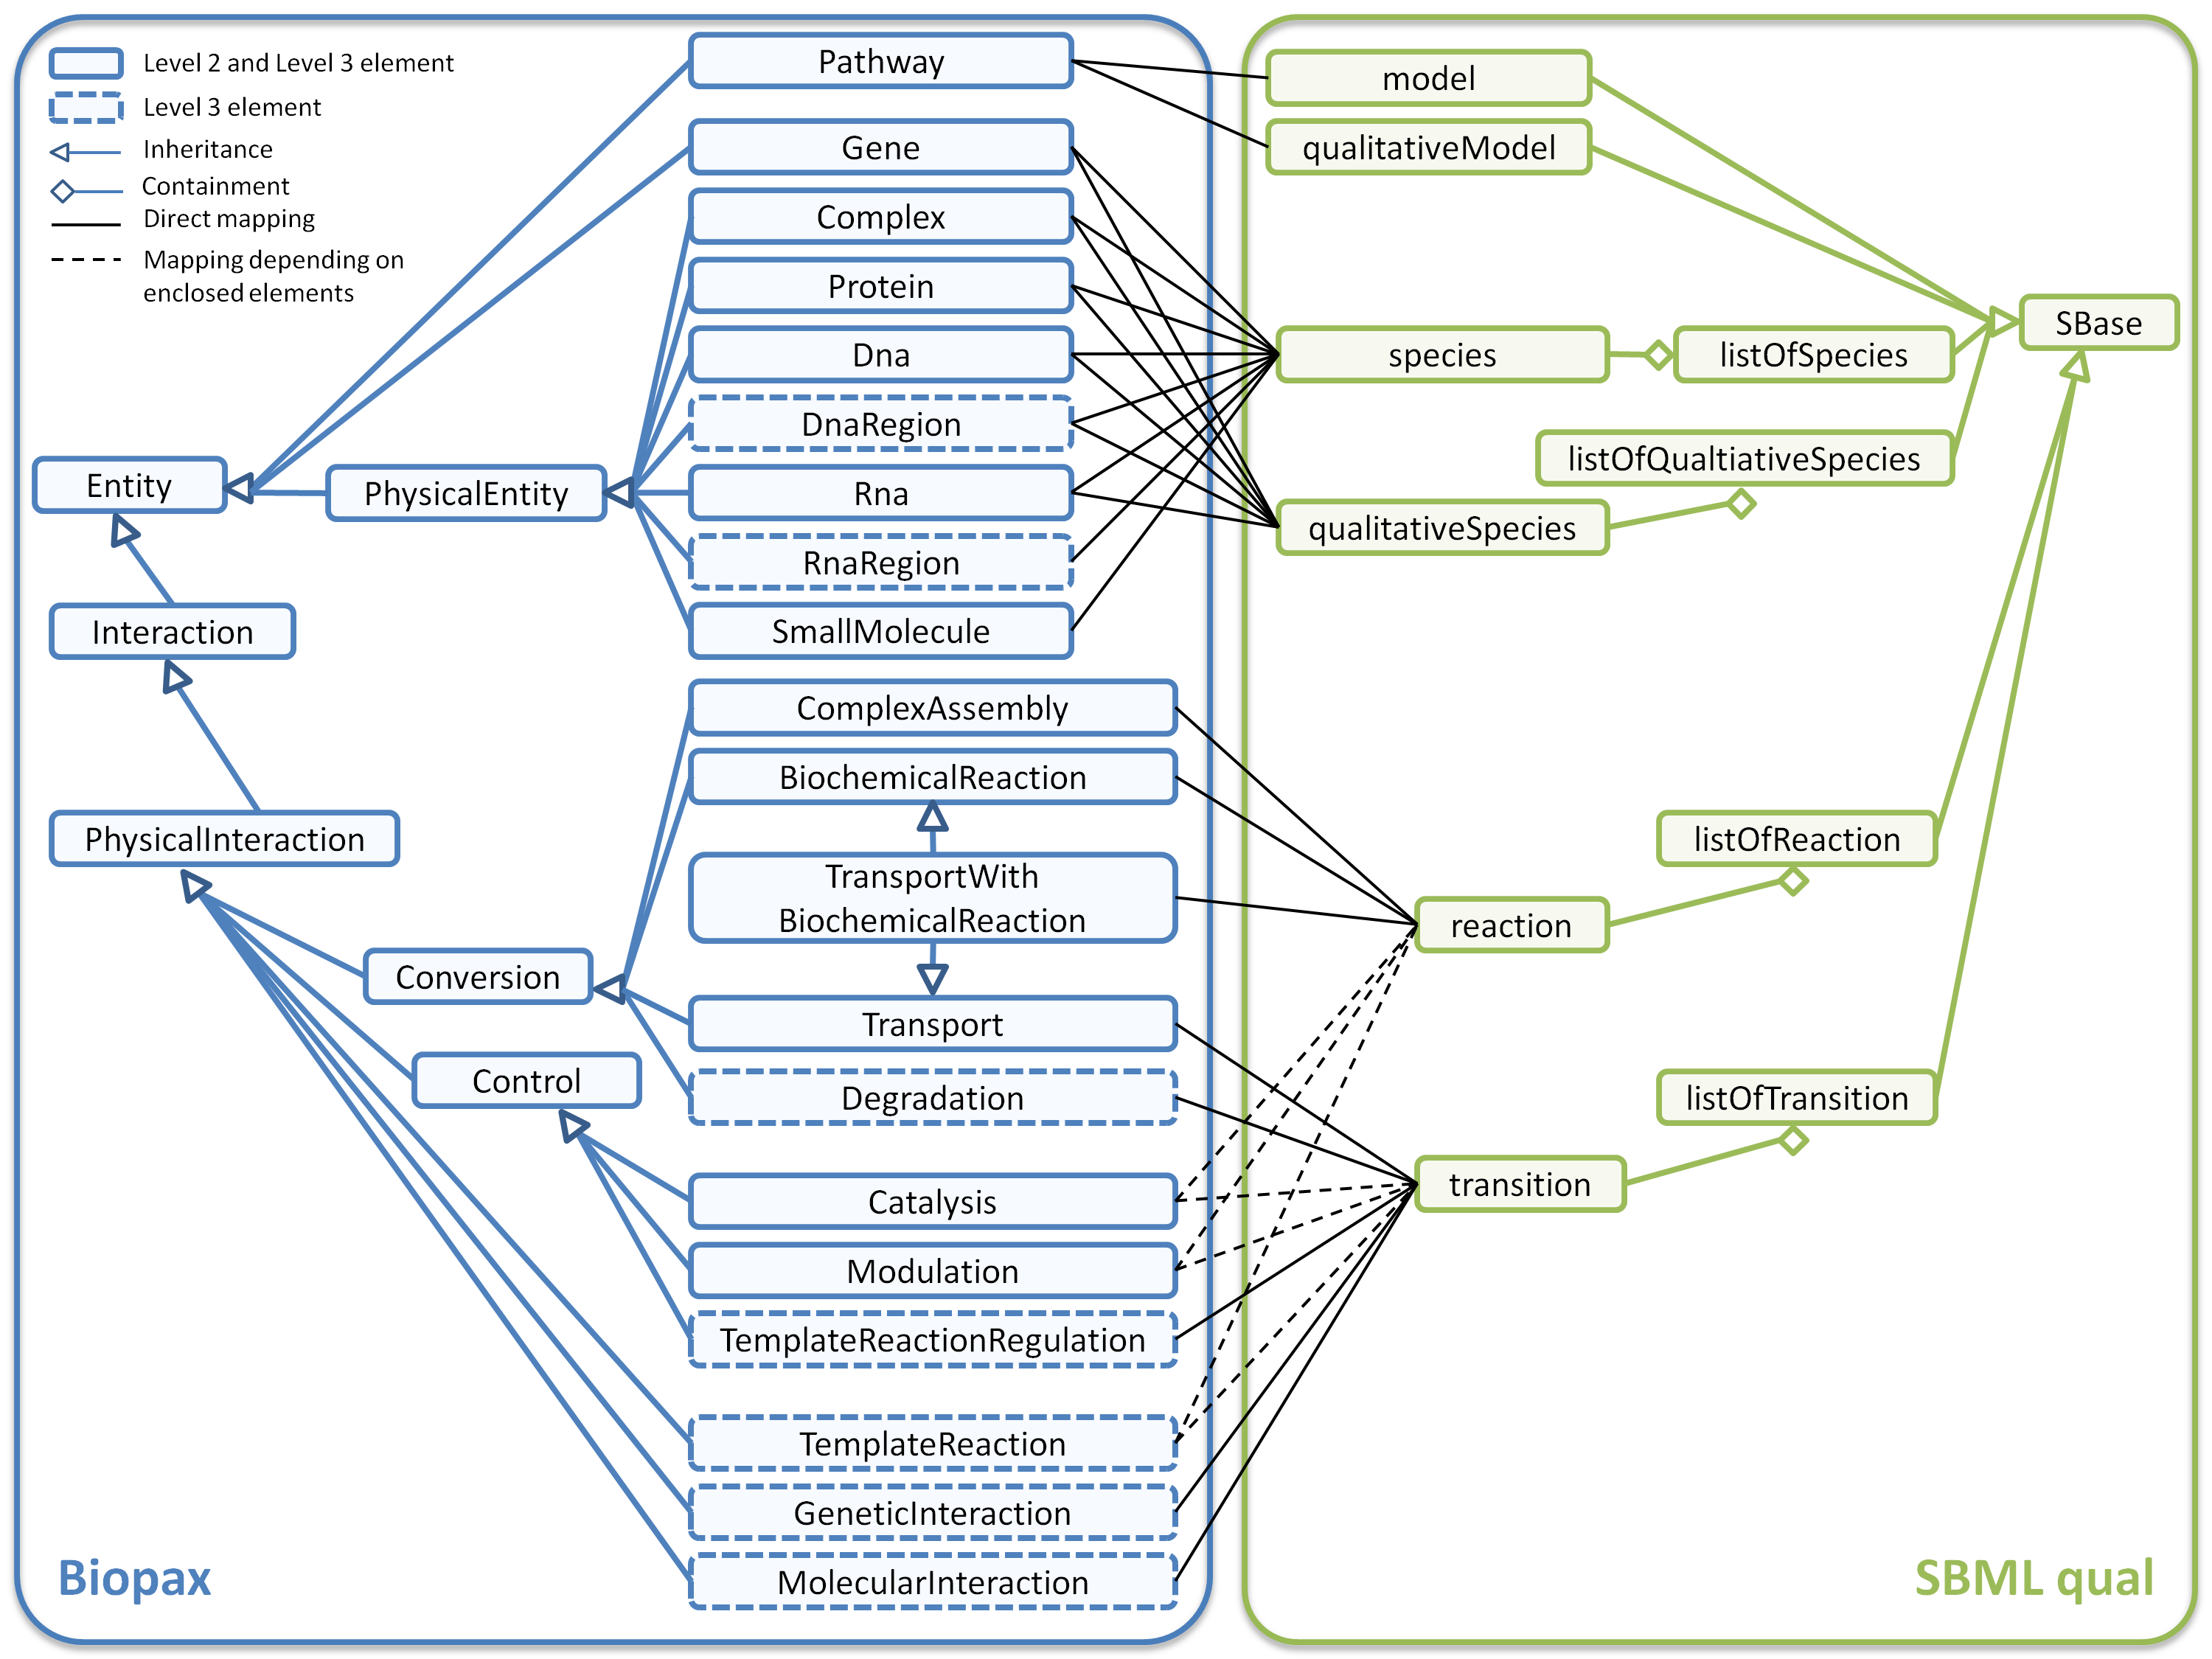
\includegraphics[width=0.96\textwidth]{BioPaxSBMLqual.png}
\caption{Conversion from BioPax Level 2 and Level 3 to SBML with the qualitative models extension (qual). The green rounded rectangles describe the SBML and SBML qual classes, and the blue ones the BioPax elements. The distinction between BioPax Level 2 and Level 3 elements is visualized with dashed rectangles. These dashed rectangles denotes Level 3 elements which are not used in Level 2. All other elements occur in both levels. The ancestry of both BioPax and SBML elements is drawn as blue arrows for BioPax respectively with green arrows for SBML. The conversion from BioPax to SBML qual is drawn with black lines. For some BioPax elements, it depends on the enclosed entities if the BioPax element is translated to a reaction or to a relation. This translation dependency is visualized with black dashed lines. A detailed translation description of these elements is shown in Table \ref{Tab:BioPax2SBML}.}\label{fig:BioPaxSBMLqual}
\end{figure*}

%\begin{figure*}[t!h]
%\centering 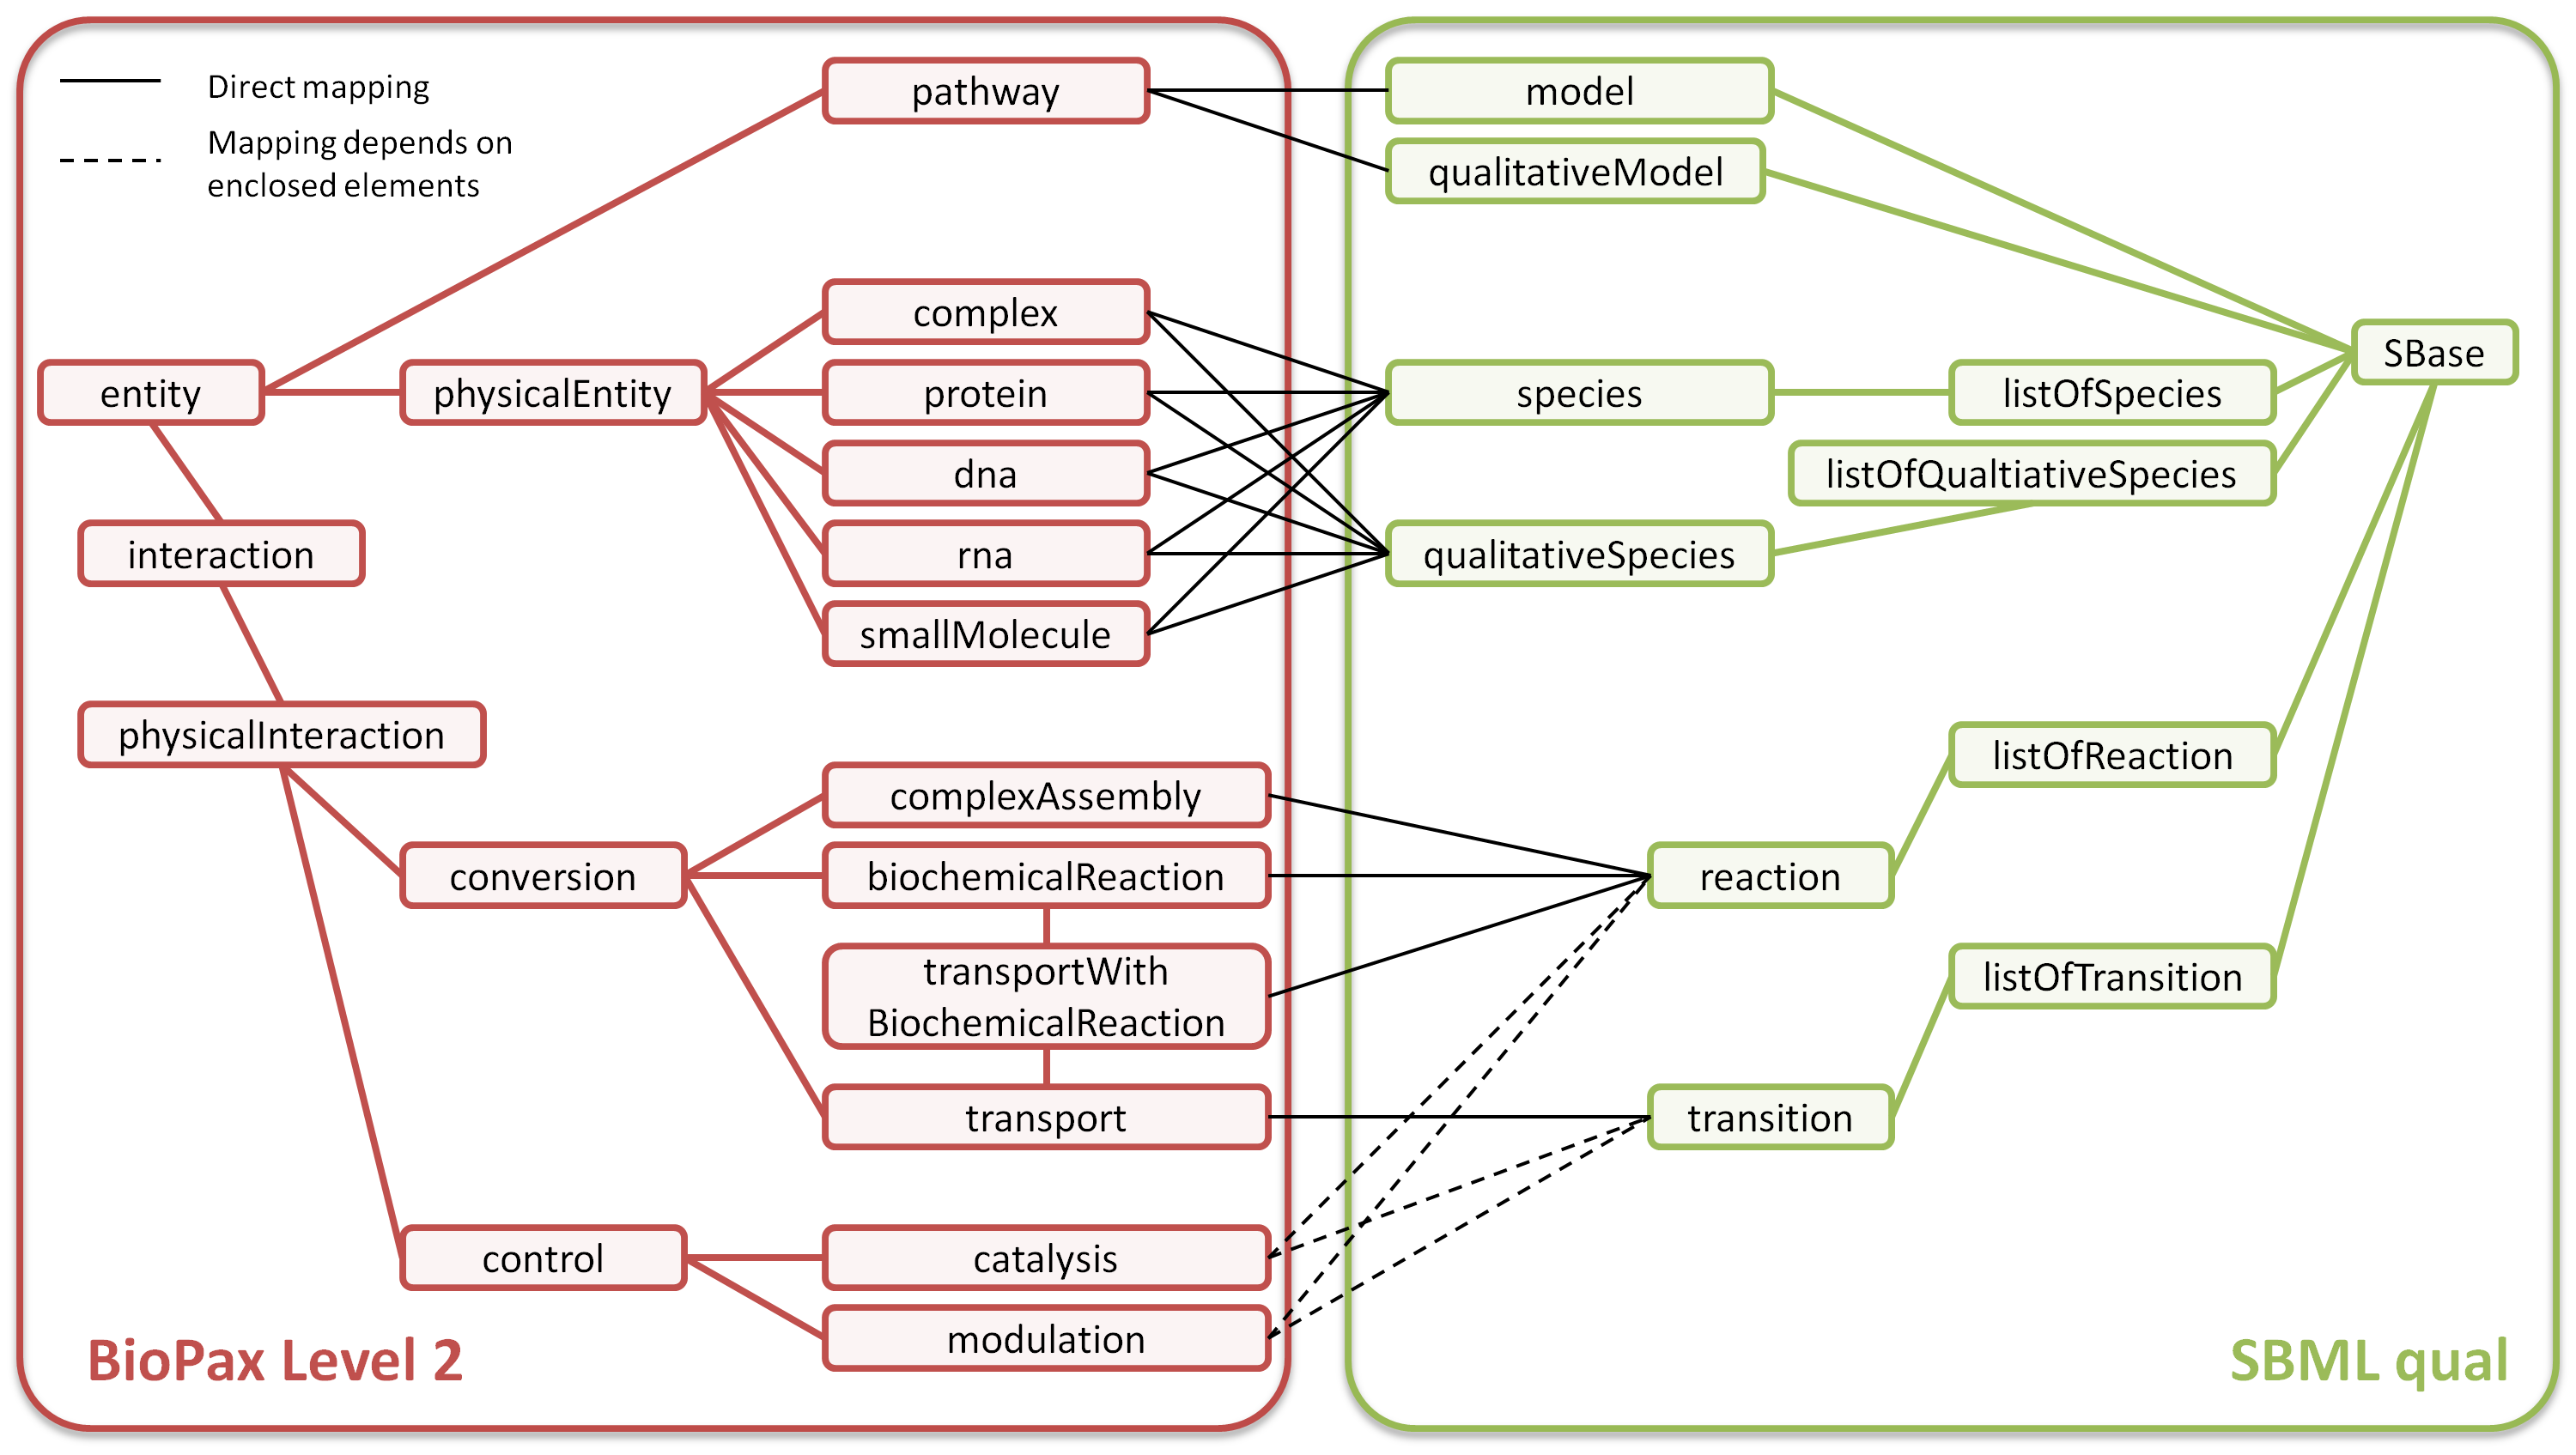
\includegraphics[width=0.96\textwidth]{BioPax2SBMLqual.png}
%\caption{Mapping from BioPax Level 2 data structures to SBML with the qualitative model extension (qual). The red rounded rectangles and lines describe the BioPax Level 2 elements and their ancestry. SBML qual entities and inheritance lines are colored green. The conversion from BioPax Level 2 to SBML qual is denoted with black lines. For some elements, it depends on the enclosed element entities if BioPax is translate to a reaction or a relation. These are visualized as black dashed lines. The translation of these elements is shown in more detail in Table \ref{Tab:BioPax2SBML}.}\label{fig:BioPax2SBMLqual}
%\end{figure*}
%
%
%\begin{figure*}[t!h]
%\centering 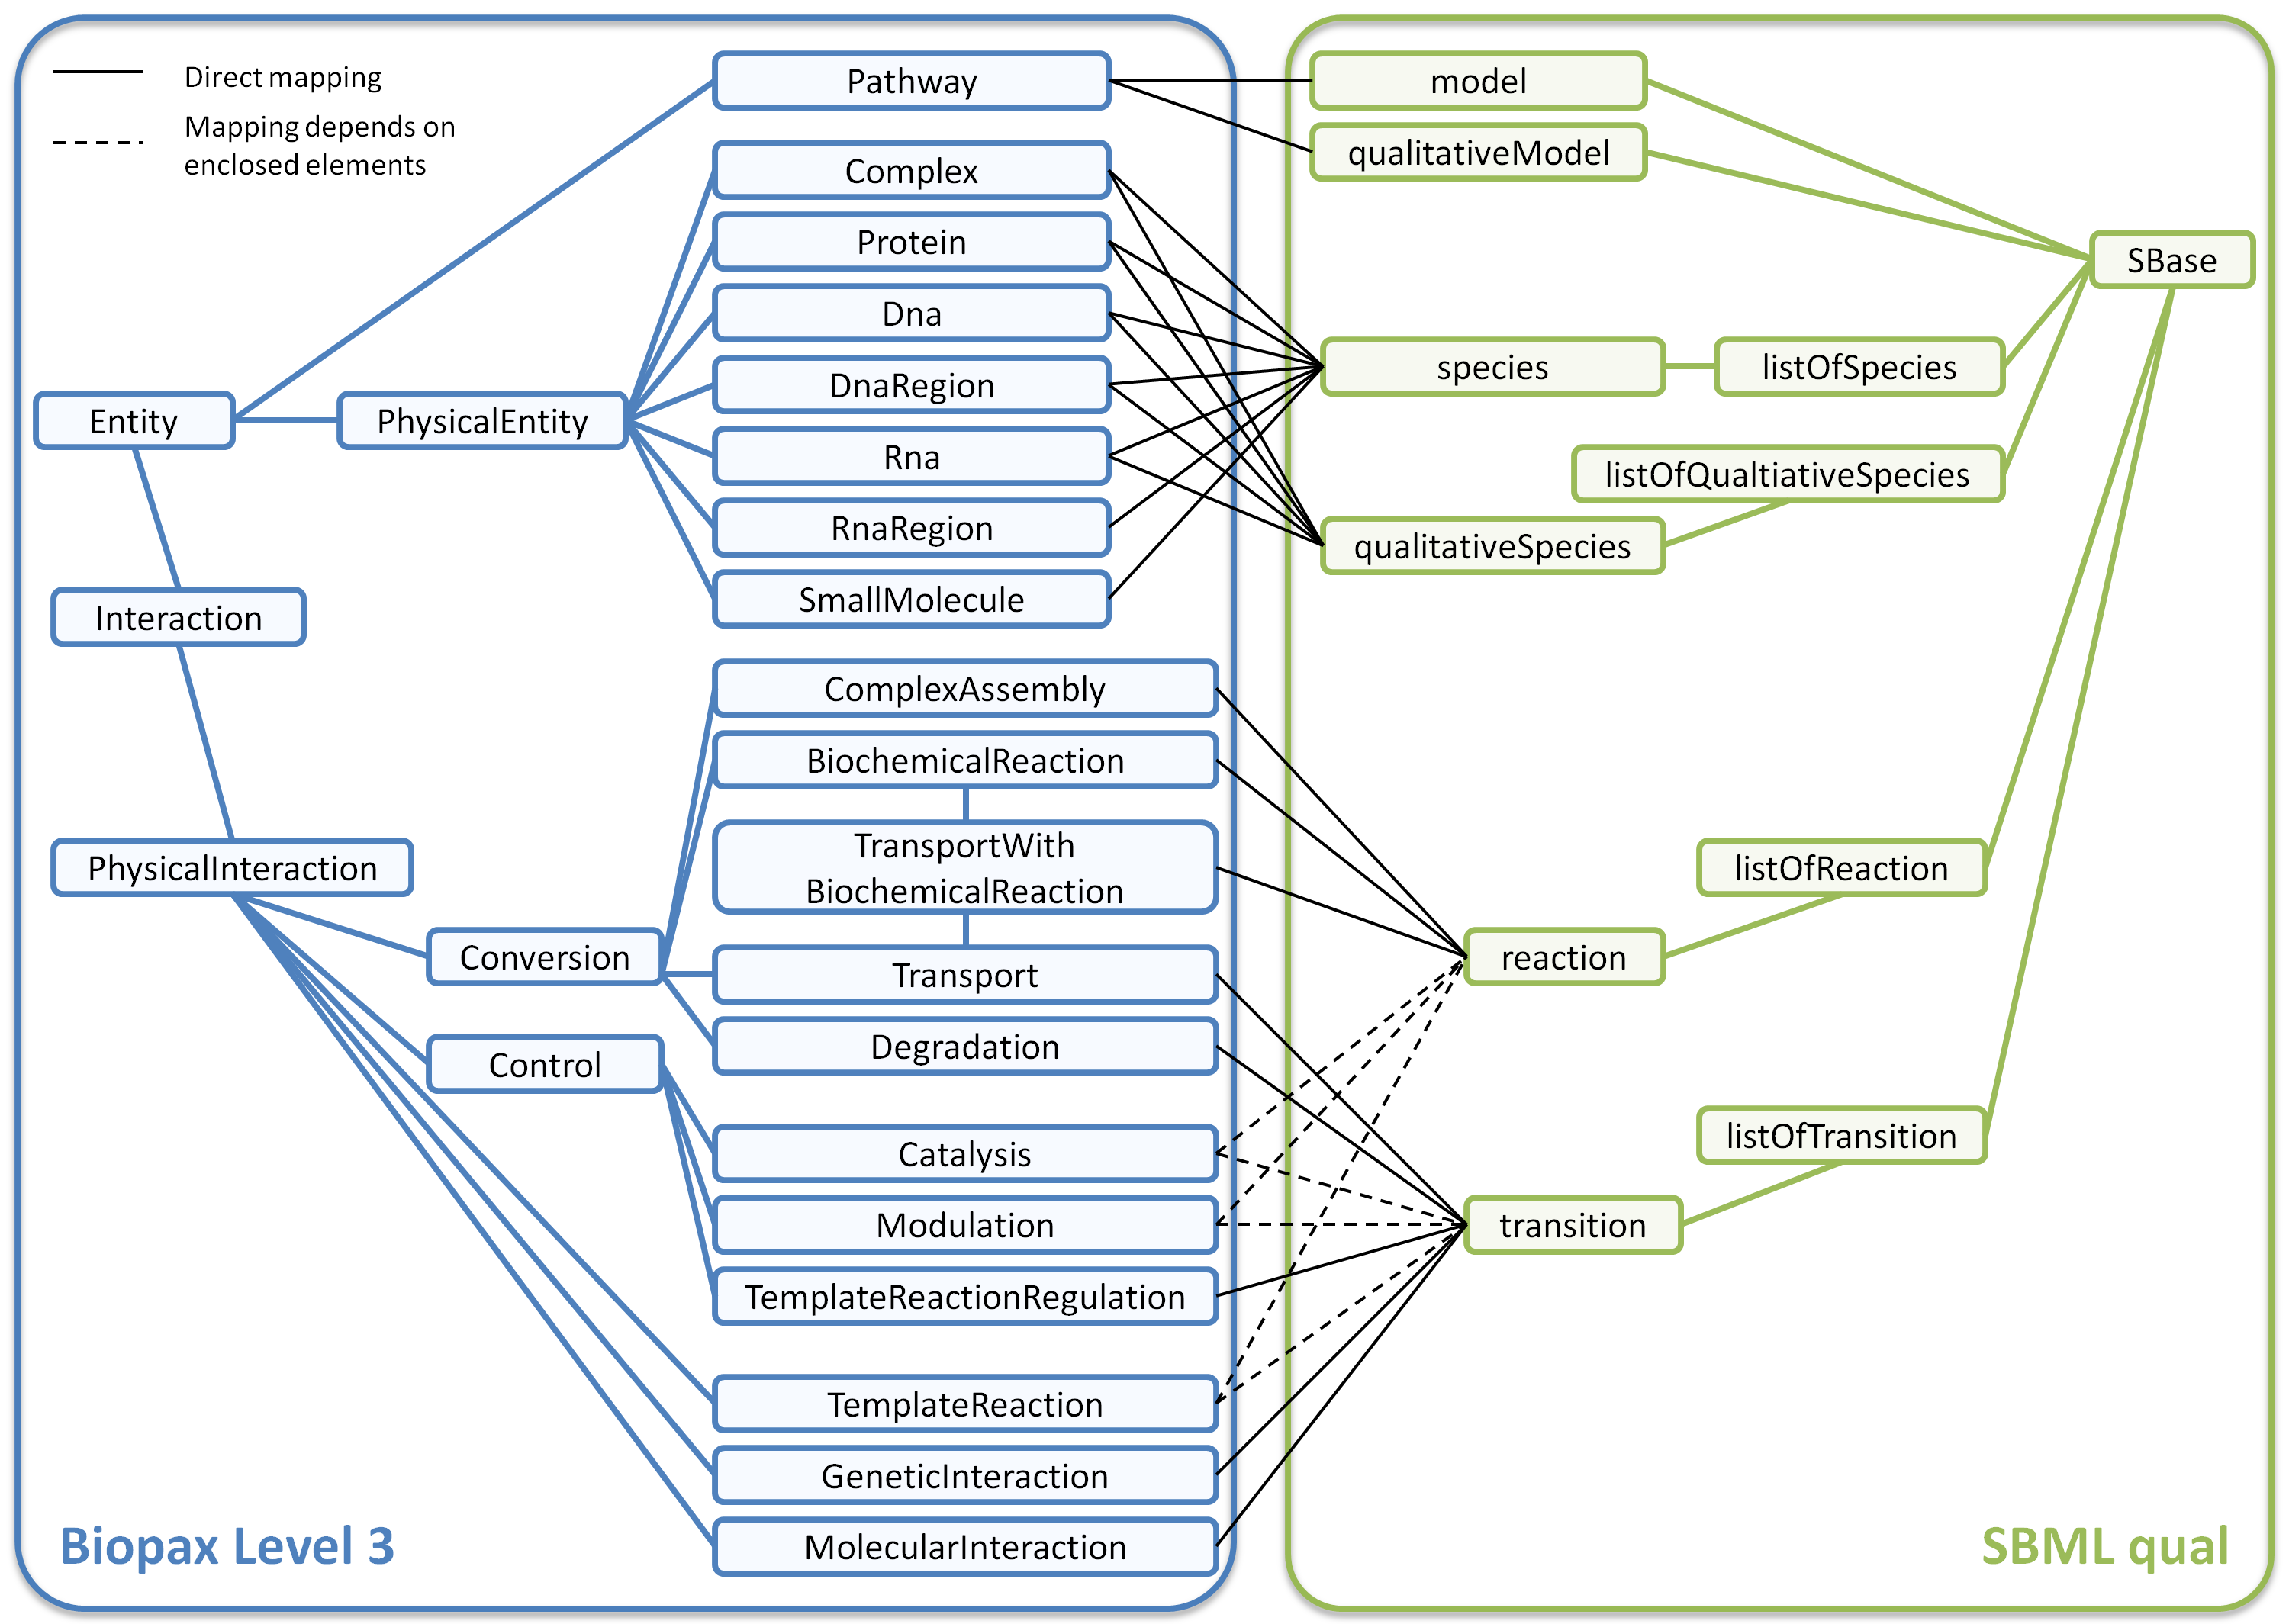
\includegraphics[width=0.96\textwidth]{BioPax3SBMLqual.png}
%\caption{Conversion from BioPax Level 3 to SBML with the qualitative model extension (qual). The blue rounded rectangles and lines describe the BioPax Level 3 elements and how they are inherited. SBML qual entities and inheritance lines are colored green. The conversion from BioPax Level 3 to SBML qual is denoted with black lines. For some elements, it depends on the enclosed element entities if BioPax is translate to a reaction or a relation. These are visualized as black dashed lines. The translation of these elements is shown in more detail in Table \ref{Tab:BioPax2SBML}.}\label{fig:BioPax3SBMLqual}
%\end{figure*}


\begin{itemize}
\item TODO: Conversion/Control elemente nochmal zus�tzlich einzeichnen?
\item Eine example conversion einbauen? -> evtl bei results and discussion um zu zeigen, warum nicht alle relationen einwandfrei \"ubersetzt werden k\"onnen
\end{itemize}
\end{methods}


\section{Results and Discussion}
%http://pid.nci.nih.gov/about.shtml#pid link for citation purposes
Warum ist es so toll einen converter von biopax to sbml qual zu haben?
\begin{itemize}
\item we can exchange and combine information from different databases using different model languages
\item \textbf{TODO: Clemens, Florian und Andreas: Habt ihr hier noch konkrete Erg\"anzungen?}
\end{itemize}

\section{Conclusion}

Conversions between different formats are important in all parts of computer sciences. Many conversions, in general, have errors or come with loss of information. The BioPax to SBML conversion is such an example. Due to limitations of the SBML specification, it was simply not possible to include all information from BioPax files in SBML files, while producing correct SBML code. But with SBML level 3 and the addition of extensions to the specifications, in particular the \texttt{qual} extension, it is now possible to create accurate and specification conform SBML code, and minimize or even eliminate the loss of information.

BioPax is an RDF format that defines various derived entities that can be genes, proteins, small molecules, etc. These can be translated to SBML species and the type of the entity can be encoded as SBO term or MIRIAM annotation on the species itself. Relations between entities (which correspond to edges in a pathway picture) are also provided with detailed information in BioPax. These can be transports, biochemical reactions, complex assemblies, etc. And this is the point where most conversions to SBML usually produce errors or have a massive loss of information. The SBML core specification only provides reactions, which represent real biochemical reactions with substrates, products and enzymes. But processes like the transport or modulation of an entity can not directly be encoded as a reaction, at least without knowing the exact chemical equation. Hence, former conversions from BioPax to SBML did either convert those relations to incorrect reactions or simply remove them during translation. To fill this gap, the SBML community has very recently released the \texttt{qual} specification, which allows to model arbitrary transitions between species. Using this extension, we produce error-free SBML and minimize or even eliminate the loss of information during the translation.

The SBML models provided with this publication consist of SBML-species and, wherever possible, exact reaction equations. Furthermore all relations from the BioPax documents that could not be converted to exact reactions have been included as qualitative transitions between the species. Additional information, like various identifiers or the type of an entity, are encoded as SBO terms or MIRIAM URNs of the corresponding elements. Furthermore, many information are added beyond the scope of the BioPax document by utilizing the KEGG API.

This results in comprehensive and correct SBML models, created for all pathways in the nature pathway interaction database, that can be downloaded from \href{http://TODO_INSERT_HOMEPAGE_HERE.de}{http://TODOINSERTHOMEPAGEHERE.de}. These models can easily be used, e.g., for further simulation and modeling steps, without having to deal with incorrect input file formats or error-prone conversions.

%TODO (DONE): mehr details von sbml core reations und qual relations und zusammenfassung der uebersetzung, inklusive MIRIAM annotations, sbo terms, etc. Letztendlich auf konvertierte pathways (+URL) als ultimatives ergebnis hinweisen.

\begin{itemize}
\item we provide a conversion from the most important database formats
\item we can exchange and combine information from different databases using different model languages
\item \textbf{TODO: Clemens, Florian und Andreas: Habt ihr hier noch konkrete Erg\"anzungen?}
\end{itemize}


\section*{Acknowledgement}
We thank xy.

\paragraph{Funding\textcolon} German Federal Ministry of Education and Research (BMBF) [National Genome Research Network (NGFN+) under grant number 01GS08134]. \textbf{TODO Virtual liver}

\bibliographystyle{natbib}
%\bibliographystyle{achemnat}
%\bibliographystyle{plainnat}
%\bibliographystyle{abbrv}
%\bibliographystyle{bioinformatics}
%\bibliographystyle{plain}
%
\bibliography{document}




\end{document}
